\documentclass[12pt]{article}

\title{ET4340 Electronics for Quantum Computing\\Homework 5}
\author{
    Mick van Gelderen\\4091566
}
\date{December 2013}

\usepackage[utf8]{inputenc}
\usepackage[a4paper,margin=2.2cm]{geometry}
\usepackage{natbib}
\usepackage{graphicx}
\usepackage{listings}
\usepackage{framed}
\usepackage{mathtools}
\usepackage{braket}
\usepackage{ifmtarg}
\usepackage{multirow}
\usepackage{xfrac}
\usepackage{xcolor}
\usepackage{caption}
\usepackage{subcaption}
% Flat UI colors MUAHAHA

\definecolor{turquoise}{HTML}{1ABC9C}
\definecolor{emerland}{HTML}{2ECC71}
\definecolor{peter-river}{HTML}{3498DB}
\definecolor{amethyst}{HTML}{9B59B6}
\definecolor{wet-asphalt}{HTML}{34495E}
\definecolor{green-sea}{HTML}{16A085}
\definecolor{nephritis}{HTML}{27AE60}
\definecolor{belize-hole}{HTML}{2980B9}
\definecolor{wisteria}{HTML}{8E44AD}
\definecolor{midnight-blue}{HTML}{2C3E50}
\definecolor{sun-flower}{HTML}{F1C40F}
\definecolor{carrot}{HTML}{E67E22}
\definecolor{alizarin}{HTML}{E74C3C}
\definecolor{clouds}{HTML}{ECF0F1}
\definecolor{concrete}{HTML}{95A5A6}
\definecolor{orange}{HTML}{F39C12}
\definecolor{pumpkin}{HTML}{D35400}
\definecolor{pomegranate}{HTML}{C0392B}
\definecolor{silver}{HTML}{BDC3C7}
\definecolor{asbestos}{HTML}{7F8C8D}

\lstset{
        language=Matlab,                                % choose the language of the code
%       basicstyle=10pt,                                % the size of the fonts that are used for the code
        numbers=left,                                   % where to put the line-numbers
        numberstyle=\footnotesize,                      % the size of the fonts that are used for the line-numbers
        stepnumber=1,                                           % the step between two line-numbers. If it's 1 each line will be numbered
        numbersep=5pt,                                  % how far the line-numbers are from the code
        backgroundcolor=\color{clouds},          % choose the background color. You must add \usepackage{color}
        showspaces=false,                               % show spaces adding particular underscores
        showstringspaces=false,                         % underline spaces within strings
        showtabs=false,                                         % show tabs within strings adding particular underscores
%       frame=single,                                           % adds a frame around the code
        tabsize=2,                                              % sets default tabsize to 2 spaces
%       captionpos=b,                                           % sets the caption-position to bottom
        breaklines=true,                                        % sets automatic line breaking
        breakatwhitespace=false,                        % sets if automatic breaks should only happen at whitespace
        escapeinside={\%*}{*)}                          % if you want to add a comment within your code
}

\newcommand{\pauli}[1]{
    \ensuremath{
        \begin{bmatrix}
            \if#1x
                0 & 1 \\
                1 & 0 \\
            \fi\if#1y
                0 & -i \\
                i & 0 \\
            \fi\if#1z
                1 & 0 \\
                0 & -1 \\
            \fi
        \end{bmatrix}
    }
}

\setlength{\parindent}{0cm}

\newcommand{\paulisigma}[1]{%
    \ensuremath{\sigma{}_{#1}}%
}

\newcommand{\bmat}[1]{\begin{bmatrix}#1\end{bmatrix}}
\newcommand{\rsqrt}[1]{\ensuremath{\frac{1}{\sqrt{#1}}}}

\setlength{\parskip}{0.5em plus4mm minus3mm}
\newenvironment{answer}{\begingroup\setlength{\leftskip}{-\leftmargin}\begin{framed}}{\end{framed}\endgroup}

\newcommand{\CNOT}[1]{\ensuremath{\texttt{CNOT}_{#1}}}
\newcommand{\CPHASE}[1]{\ensuremath{\texttt{CPHASE}_{#1}}}
\newcommand{\SWAP}[1]{\ensuremath{\texttt{SWAP}_{#1}}}
\newcommand{\cnotgr}[1]{\ensuremath{\bmat{%
        1 & 0 & 0 & 0 \\%
        0 & 1 & 0 & 0 \\%
        0 & 0 & 0 & 1 \\%
        0 & 0 & 1 & 0 \\%
}}}

\begin{document}

\maketitle

\paragraph{Problem 1: Warmup exercises} \hfill

\begin{enumerate}
    \item Consider an operator $M$ and one of its eigenstates $\ket{\psi}$ (with eigenvalue $\lambda$). Consider another operator $A$ that anticommutes with $M$ (i.e., $\{M,A\} \equiv MA + AM = 0$). Show that the state $A\ket{\psi}$ is an eigenstate of $M$ with eigenvalue $-\lambda$.

    \begin{answer}
        We can write $M\ket{\psi} = \lambda\ket{\psi}$.
        \begin{align*}
            MA + AM &= 0 \\
            MA\ket{\psi} + AM\ket{\psi} &= 0 \\
            MA\ket{\psi} + A\lambda\ket{\psi} &= 0 \\
            M\left(A\ket{\psi}\right) &= -\lambda\left(A\ket{\psi}\right) \\
        \end{align*}
    \end{answer}

    \item Now consider an operator $B$ that commutes with $M$ (i.e., $[M,B] \equiv MB - BM = 0$). Show that the state $B\ket{\psi}$ is an eigenstate of $M$ with eigenvalue $\lambda$.

    \begin{answer}
        Assuming M again has an eigenstate $\ket{\psi}$ with eigenvalue $\lambda$.
        \begin{align*}
            MB - BM &= 0 \\
            MB\ket{\psi} - BM\ket{\psi} &= 0 \\
            M\left(B\ket{\psi}\right) &= \lambda\left(B\ket{\psi}\right) \\
        \end{align*}
    \end{answer}

    \item Prove the identity:

    \begin{center}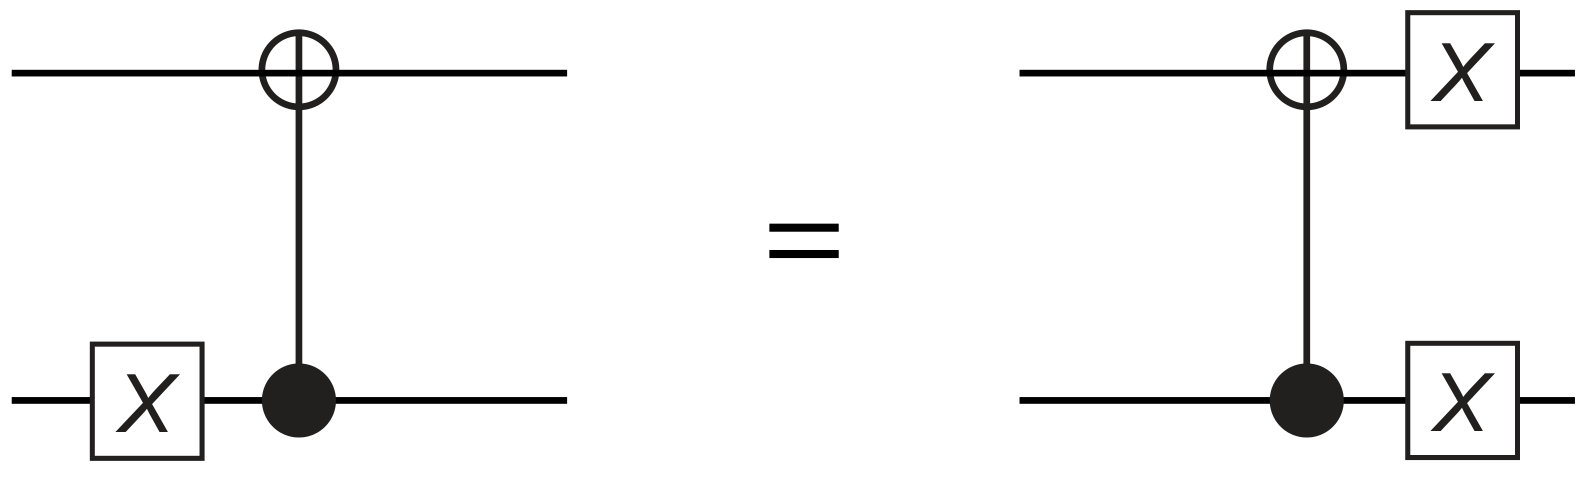
\includegraphics[width=.8\textwidth]{problem-1.png}\end{center}

    Feel free to do this either by multiplying matrices or by manipulating circuit diagrams. From this we see that a single-qubit bit-flip error prior to \CNOT{} proliferates into a double bit-flip error.

    \begin{answer}
        It is an intuitive identity in my opinion. Flipping the control bit flips the output. So to `simulate' the flip before a \CNOT{} you can flip both the output and the control after the \CNOT{}.

        By matrice multiplication (note that the order of operations is reversed with respect of the diagram because we compute the combined matrix $M = M_n\dots{}M_2M_1$ in $\ket{out} = M\ket{in}$ where $M_n$ is operation $n$):

        \begin{align*}
            M_a &= \CNOT{01}(I \otimes X) &=
                \bmat{1&0&0&0\\0&0&0&1\\0&0&1&0\\0&1&0&0}
                \bmat{0&1&0&0\\1&0&0&0\\0&0&0&1\\0&0&1&0} &=
                \bmat{0&1&0&0\\0&0&1&0\\0&0&0&1\\1&0&0&0}\\
            M_b &= (X \otimes X)\CNOT{01} &=
                \bmat{0&0&0&1\\0&0&1&0\\0&1&0&0\\1&0&0&0}
                \bmat{1&0&0&0\\0&0&0&1\\0&0&1&0\\0&1&0&0} &=
                \bmat{0&1&0&0\\0&0&1&0\\0&0&0&1\\1&0&0&0}\\
            M_a &= M_b
        \end{align*}
    \end{answer}
\end{enumerate}

\paragraph{Problem 2: Three-qubit bit flip code} \hfill

Consider the 3-qubit bit-flip code as covered in the lectures. In this code, a one-qubit state $\ket{\psi} = \alpha\ket{0_2} + \beta\ket{1_2}$ is encoded as $\ket{\Psi} = \alpha\ket{0_30_20_1} + \beta\ket{1_31_21_1}$.

\begin{enumerate}
	\item Suppose the encoded state is distorted by a rotation of $60\deg$ about the $+\hat{x}$ axis of qubit 3. What are the possible error syndromes you could measure (i.e., the measurement results $m_a$ and $m_b$)? Show that the state $\ket{\Psi}$ is recovered after error correction, every time.

	\begin{answer}
		Since the distortion is not a full flip you can measure qubit 3 as either $-1$ or $+1$. The other two bits are not affected and will retain their (equal) states.

		The $Z$ (parity) measurement $m_a$ of qubits $q_1$ and $q_2$ will always give $m = -1$ because $q_1 = q_2$. Since the same does not hold for qubit $q_3$ you will measure $m = \pm1$.

		The error syndromes thus are $m_a = -1, m_b = -1$ and $m_a = -1, m_b = +1$. In the first case you won't have to do anything. In the second case you will have to flip qubit $q_3$ back.
	\end{answer}

	\item Suppose now that instead the encoded state is distorted by a rotation of $45\deg$ about the $+\hat{y}$ axis of qubit $q_2$, but you don't know it and stick to using the bit flip code without modifications. What are the possible error syndromes you would measure? Can you recover the state $\ket{\Psi}$ every time? When do you succeed and when do you not? When you don't recover it, what is the erroneous final state of the logical qubit?

	\begin{answer}
		This time we apply a maybe-$Y$ gate to qubit $q_2$. Since $Y = iXZ$ and the measurements we perform are two $Z$ measurement, we can make some conclusions about the different cases.

		We can recover the error when the state becomes $X\ket{\Psi}$ because the syndrome is $m_a = -1, m_b = -1$. I
	\end{answer}

\end{enumerate}


\end{document}

